\documentclass{article}
\usepackage[utf8]{inputenc}
\usepackage[portuges]{babel}
\usepackage{csquotes}
\usepackage{geometry}
\usepackage{indentfirst}
\usepackage{graphicx}
\usepackage{float}
\usepackage[pdftex]{hyperref}
\usepackage[backend = biber]{biblatex}
\addbibresource{referencias.bib}
\geometry{top = 3cm, bottom = 2cm, left = 3cm, right = 2cm}

\title{Banco de Dados}
\author{Igor Cortes Junqueira \\ Igor Patrício Michels}
\date{2020.2}

\begin{document}

\maketitle

\section{Introdução}

O presente documento tem por objetivo relatar o desenvolvimento da elaboração da visualização em grafo de um banco de dados para a segunda avaliação da disciplina de Banco de Dados da FGV-EMAp, ministrada pelo professor Renato Rocha Souza. O objetivo é realizar a visualização em grafo do banco de dados desenvolvido na primeira avaliação com informações sobre os voos domésticos dos EUA entre janeiro de 2019 e maio de 2020, cujos scripts podem ser encontrados em \cite{github} e o banco pode ser encontrado \href{https://gvmail-my.sharepoint.com/:f:/g/personal/b39254_fgv_edu_br/Ev8i0xwOqnFFh_q3gTqvNAkBhzL_dpV6_ljzh82vJsTnNg?e=7ubrsl}{\textbf{nesse link}}. Já o desenvolvimento do presente trabalho pode ser encontrado em \cite{github2}.

\section{Elaboração}

\subsection{Fontes}

Como estamos utilizando o banco desenvolvido no trabalho anterior, as fontes dos dados dos voos utilizados se mantém, ou seja, os dados dos voos foram obtidos por meio dos registros oficiais da BTS - Bureau of Transportation Statistics \cite{BTS}, já os dados das aeronaves foram obtidos pelos registros da FAA - Federal Aviation Administration \cite{FAA}.

\subsection{Modelo Lógico}

Para realizar a manipulação dos dados é super válido relembrar a estrutura lógica do banco para que facilite no momento em que formos realizar query's. Dessa forma, conforme relatório passado, o modelo lógico final é o seguinte:

\begin{figure}
    \centering
    \includegraphics[scale = 0.7]{Imagens/modelo lógico.png}
    \caption{Modelo Lógico}
    \label{lógico}
\end{figure}

\subsection{Desenvolvimento}

Nosso primeiro passo foi elaborar um grafo básico com as companhias aéreas apontando para as rota que possuem, por exemplo, a Hawaiian Airlines INC possui, entre suas rotas, as rotas de Honolulu a Kuhului (rota HNL-OGG) e de Kuhului a Honolulu (rota OGG-HNL), teremos um nó que representa a companhia com uma aresta apontando para um nó que representa a rota HNL-OGG e também uma outra aresta que aponta para um nó representando a rota OGG-HNL. No fim, obtivemos o seguinte grafo:
\begin{figure}
    \centering
    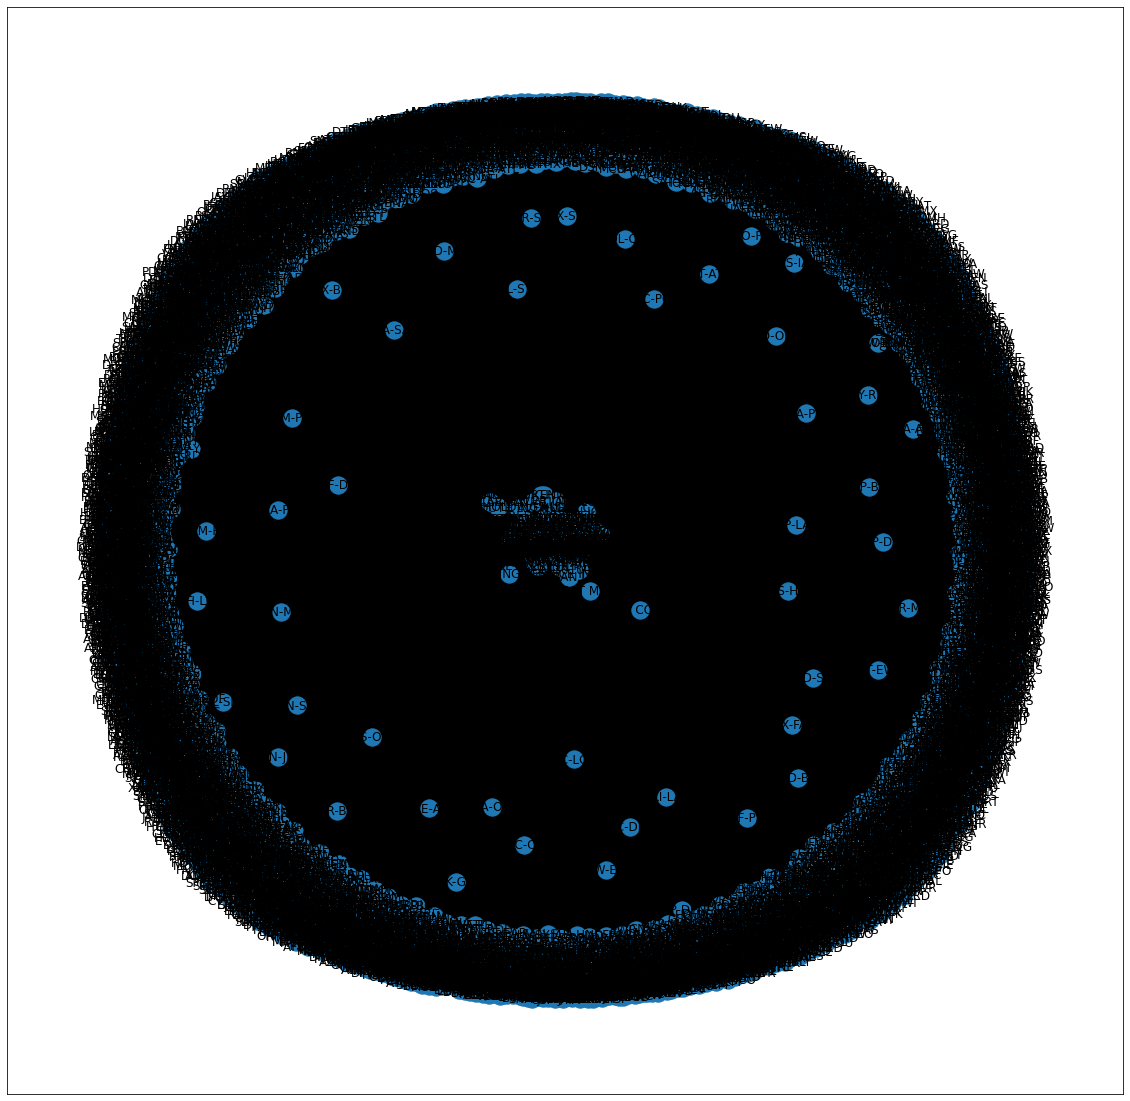
\includegraphics[scale = 0.3]{Imagens/todos.png}
    \caption{Grafo com todas as companhias e rotas}
    \label{grafo}
\end{figure}

Conforme podemos notar na Imagem \ref{grafo}, não conseguimos extrair informação alguma de um grafo com todas informações disponíveis ao mesmo tempo pois o mesmo acaba ficando poluído. Dessa forma elaboramos algumas restrições quanto as companhias e os aeroportos, selecionando apenas os dez aeroportos mais movimentados\footnote{Com maior volume de voos.} junto das seis maiores companhias\footnote{Também em volume de voos.}, obtendo o grafo que pode ser visto na Figura \ref{preview}, o qual já nos traz informações relevantes.
\begin{figure}
    \centering
    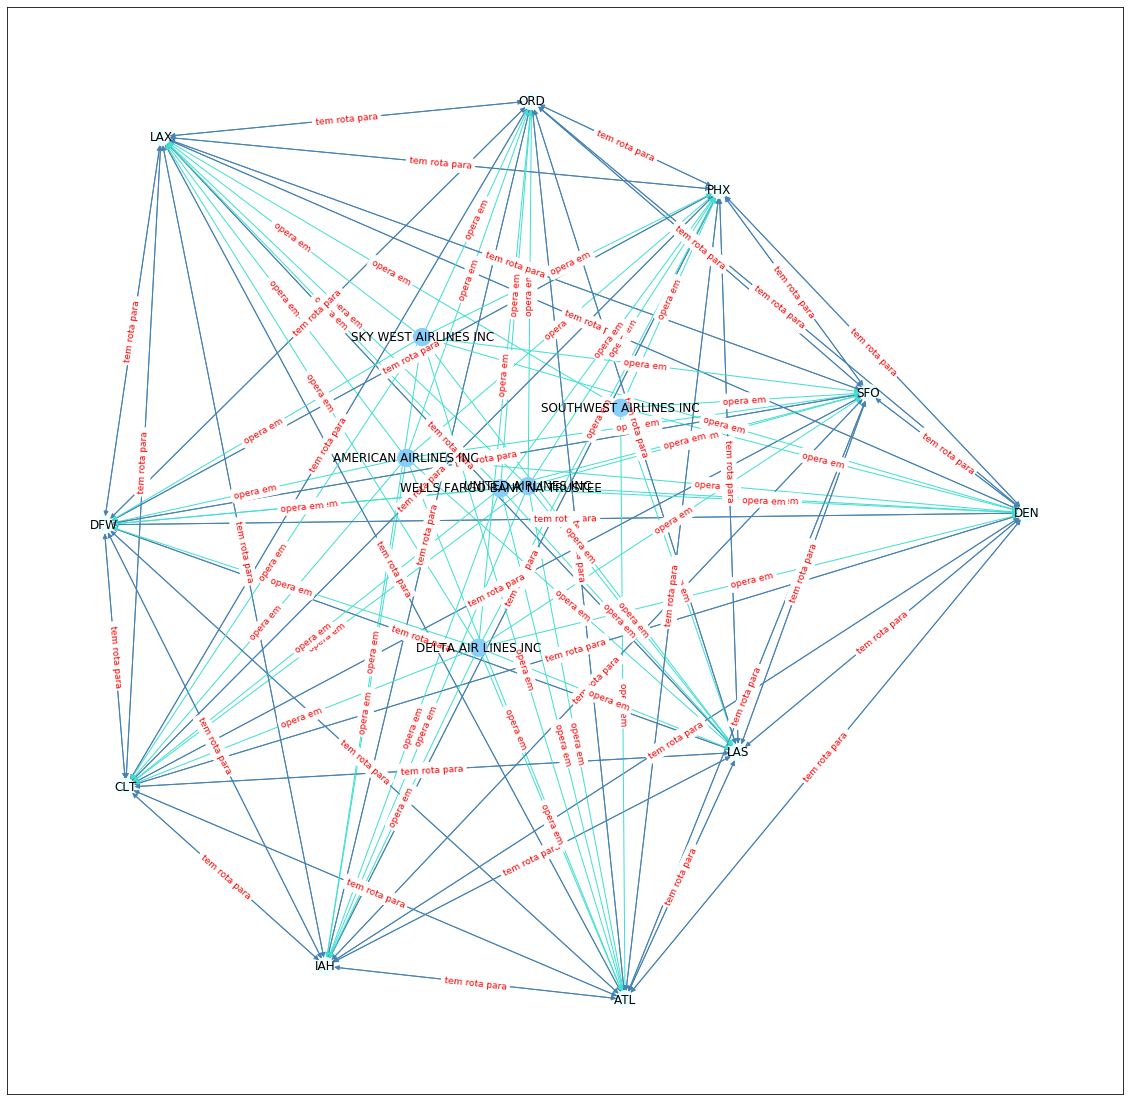
\includegraphics[scale = 0.3]{Imagens/preview.png}
    \caption{Grafo mais limpo das companhias e rotas}
    \label{preview}
\end{figure}




\section{Resultados}















\printbibliography

\end{document}
